
\documentclass[11pt, a4paper]{book}
\usepackage[french]{babel}
\usepackage[utf8]{inputenc}
\usepackage{answers}

\usepackage{hyperref}
\usepackage{multicol}

\usepackage[table,xcdraw]{xcolor}
\usepackage{listings}
\definecolor{ForestGreen}{RGB}{34,139,34}


\usepackage{enumitem}

\AtBeginDocument{\def\labelitemi{$\bullet$}}


\newcommand{\py}{\lstinline{Python} }


\definecolor{backcolour}{rgb}{0.95,0.95,0.92}

\lstset{%
	language         = Python,
	backgroundcolor  = \color{backcolour},
	basicstyle       = \ttfamily, % \upshape\ttfamily,
	keywordstyle     = \bfseries\color{blue}, %\bfseries,
	stringstyle      = \color{magenta},
	commentstyle     = \color{ForestGreen},
	alsoletter = > ,
	morekeywords = {>>>,as,assert,False,None, nonlocal,True, with,yield , <<, >>, :},
	showstringspaces = false,
	numbers=left,
	stepnumber=1,
	literate={à}{{\`{a}}}1 {é}{{\'e}}1 {è}{{\`{e}}}1 {ê}{{\^{e}}}1 {Ê}{{\^{E}}}1 {î}{{\^i}}1 {ô}{{\^{o}}}1 {ç}{{\c{c}}}1 {Ç}{{\c{C}}}1
}

\newcommand{\itemb}[1]{\item \textbf{#1}}

\usepackage{fancyhdr}  %package pour en-tetes et pied de pages
\usepackage{sectsty} % Permet de faire des modifications de police dans diverses sections des "headings" (cf. modif presentation de la page)
\pagestyle{fancy}       %Style pour en-tetes et pieds de pages
\fancyhead[CO,CE]{\sc Série 1\hspace{0.5mm}}
\fancyhead[RO,LE]{Collège Sismondi}  % LaTeX/TEX define \strut to be an invisible box of width zero that extends just enough above and below the baseline. Cela permet d'augementer légèrement la taille en bas de la box de manière à ce qu'elle soit collée à la ligne.
\fancyhead[LO,RE]{\small\ \textsl{1\textsuperscript{ère} année - DO Informatique}}
\fancyfoot[RO,LE]{2021 - 2022}
\fancyfoot[LO,RE]{\small }
\fancyfoot[CO,CE]{\thepage}

\fancyhfoffset[l]{1.2cm} % le "l" en paramètre permet d'indiquer qu'on ne veut modifier que la marge à gauche.
\renewcommand{\headrule}{{%
		\hrule \headwidth \headrulewidth \vskip-\headrulewidth}}
\renewcommand\footrulewidth{\headrulewidth}
\renewcommand{\footrule}{{%
		\vskip-\footruleskip\vskip-\footrulewidth
		\hrule \headwidth \footrulewidth\vskip\footruleskip}}

\usepackage{tikz}
%-------------------------------------------------------------------------------
%---- Eclairage : en encadré sur fond jaune avec symbôle "ampoule" à gauche ----
%-------------------------------------------------------------------------------
\definecolor{coleclairage}{RGB}{255 , 221 , 156}
\definecolor{contoureclairage}{RGB}{255 , 192 , 0}
\newenvironment{eclairage}
{
	\begin{center}%
		\begin{tikzpicture}%
			\node[rectangle, draw=contoureclairage, top color=coleclairage!50, bottom color=coleclairage!140, rounded corners=5pt, inner xsep=5pt, inner ysep=6pt, outer ysep=10pt]\bgroup                     
			\begin{minipage}{0.98\linewidth}
				\begin{minipage}{0.08\linewidth}\centerline{
\includegraphics[scale=1]{Symbole_eclairage.png}}\end{minipage}
				\begin{minipage}{0.89\linewidth}\itshape\footnotesize
				}
				{                		
				\end{minipage}
			\end{minipage}\egroup;%
		\end{tikzpicture}%
	\end{center}%
}

%-------------------------------------------------------------------------------
%---- apprendre : en encadré sur fond jaune avec symbôle "ampoule" à gauche ----
%-------------------------------------------------------------------------------
\definecolor{colapprendre}{RGB}{50,205,50}
\definecolor{contourapprendre}{RGB}{34,139,34}
\newenvironment{apprendre}
{
	\begin{center}%
		\begin{tikzpicture}%
			\node[rectangle, draw=contourapprendre, top color=colapprendre!10, bottom color=colapprendre!50, rounded corners=5pt, inner xsep=5pt, inner ysep=6pt, outer ysep=10pt]\bgroup                     
			\begin{minipage}{0.98\linewidth}
				\begin{minipage}{0.08\linewidth}\centerline{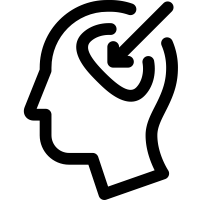
\includegraphics[width=30px]{Symbole_learn.png}}\end{minipage}
				\begin{minipage}{0.89\linewidth}\itshape\footnotesize
				}
				{                		
				\end{minipage}
			\end{minipage}\egroup;%
		\end{tikzpicture}%
	\end{center}%
}

\definecolor{colimportant}{RGB}{247 , 189 , 164}
\definecolor{contourimportant}{RGB}{237 , 125 , 49}
\newenvironment{important}
{
	\begin{center}%
		\begin{tikzpicture}%
			\node[rectangle, draw=contourimportant, top color=colimportant!50, bottom color=colimportant!140, rounded corners=5pt, inner xsep=5pt, inner ysep=6pt, outer ysep=10pt]\bgroup                     
			\begin{minipage}{0.08\linewidth}\centerline{
\includegraphics[scale=0.8]{Symbole_attention.png}}\end{minipage}
			\begin{minipage}{0.89\linewidth}
			}
			{                		
			\end{minipage}\egroup;
		\end{tikzpicture}%
	\end{center}%
}

%-----------------------------------------------------------------
%---- Modification présentation de la page: marges de la page ----
%-----------------------------------------------------------------
%\addtolength{\hoffset}{-1in}              % 1
%\addtolength{\voffset}{-1in}              % 2
\addtolength{\oddsidemargin}{-0.1 in} % 3
\addtolength{\evensidemargin}{-1in} % 3
\addtolength{\topmargin}{-1in}       % 4
\addtolength{\headheight}{6pt}       % 5
%\addtolength{\headsep}{-0.2cm}           % 6
\setlength{\textheight}{26cm}    % 7
\setlength{\textwidth}{16.5cm}      % 8
\addtolength{\marginparsep}{0pt}      % 9
\setlength{\marginparwidth}{0pt}   % 10
\addtolength{\footskip}{-1mm}           %11

\setlength{\parindent}{0em}% pas d'indentation


% Customiser le nom des sections
\usepackage{titlesec}
\titleformat{\section}[hang]{\Large \bfseries}{Série \thesection:\ }{0pt}{}

\renewcommand{\familydefault}{\sfdefault} % pour avoir des polices san serif

\newtheorem{Exc}{Exercice}
\Newassociation{correction}{Soln}{mycor}
\renewcommand{\Solnlabel}[1]{\bfseries Ex #1 }
\def\exo#1{%
	\futurelet\testchar\MaybeOptArgmyexoo}
\def\MaybeOptArgmyexoo{
	\ifx[\testchar \let\next\OptArgmyexoo
	\else \let\next\NoOptArgmyexoo \fi \next}
\def\OptArgmyexoo[#1]{%
	\begin{Exc}[#1]\normalfont}
	\def\NoOptArgmyexoo{%
		\begin{Exc}\normalfont}
		\newcommand{\finexo}{\end{Exc} \vspace{3mm}}
	\newcommand{\flag}[1]{}
	\newcommand{\entete}[1]

\newcommand{\getexocompteur}{{\the\numexpr \arabic{Exc}  \relax}}	
	
\newcommand{\eexo}{\vspace{5mm}} % espace pour séparer les exercices
\pgfplotsset{compat=1.17}
\begin{document}

\setcounter{chapter}{6}

\chapter{Programmation - Types et Variables}


\section{Quelques notions de base}

Tous les langages de programmation ont été créés dans le même but \textbf{traiter de l'information}. Dans un langage impératif, on retrouve toujours les concepts suivants : 
\begin{itemize}
	\itemb{La notion de valeur} qui représente l'information,
	\itemb{La notion d'expression} qui produit une valeur,
	\itemb{La notion d'instruction} qui est une commande à exécuter par la machine,
	\itemb{La notion de structure de contrôle} qui exécute des instructions d'une manière bien spécifique en fonction des valeurs.
\end{itemize}

\subsection{La notion de valeur}
Une valeur est une représentation de l'information. Par exemple le nombre entier \lstinline{3} représente une valeur, de même que la chaîne de caractères \lstinline{"Hello world"} ou le tableau de nombres à virgule flottante \lstinline{[7.31, 1.74, 3.14, 10.0]}  (similaire aux nombres décimaux). Une valeur est toujours associée à un type (nombre entier/virgule flottante, chaîne de caractères).\\

\subsection{La notion d'expression}
Des valeurs, des opérateurs mathématiques et des parenthèses peuvent former une expression. Une expression est évaluée et le résultat de cette évaluation donne une valeur. 
\begin{mydefinition}
	Une expression est le résultat d'un calcul effectué par le programme. Elle fournit une valeur associé à un type.
\end{mydefinition}

On peut utiliser l'interpréteur python pour évaluer des expressions
\begin{myexample}
	\begin{lstlisting}[numbers=none]
>>>(1 + 2) * (3 + 4)
21
	\end{lstlisting}
	Ici l'expression produit la valeur \lstinline{21} qui est de type entier.
\end{myexample}

\subsection{La notion d'instruction}
Une instruction peut être vue comme une commande ou un ordre que l'on donne à la machine. En Python, il y a deux types d’instruction:
\begin{itemize}
	\item affectation : qui effectue un calcul et qui le stocke en mémoire dans une variable.
	\item fonction    : qui est une "commande" prédéfinie. 
\end{itemize}
\begin{myexample}
	\vspace{-3mm}
	\begin{lstlisting}[numbers=none]
>>> x = 1 + 2       # c'est une affectation
>>> print(x)        # c'est un appel à une fonction
3
	\end{lstlisting}
	\vspace{-3mm}
\end{myexample}


\begin{eclairage}
	Tout texte qui suit le caractère dièse "\lstinline{#}" est ignoré par Python, on appelle ceci des commentaires. Leur but est d’expliquer le fonctionnement du programme. C’est une bonne habitude de commenter abondamment le code.
\end{eclairage}
Pour utiliser une instruction, par exemple la \textbf{fonction} \lstinline{print}, il faut lui fournir une valeur (l'information à afficher). Dans l'exemple
\begin{lstlisting}[numbers=none]
>>> print("I love computer science")
I love computer science
\end{lstlisting}
la valeur à afficher est le message \lstinline{"I love computer science"}. En revanche, la commande 
\begin{lstlisting}[numbers=none]
>>>print(3 * 5 + 2)
17
\end{lstlisting}
ne produit pas le même résultat que 
\begin{lstlisting}[numbers=none]
>>> print("3 * 5 + 2")
3 * 5 + 2
\end{lstlisting}
car dans le premier cas la valeur est un nombre qui est le résultat de l'évaluation de l'expression $3\cdot 5 +2$ (un nombre entier), et dans le second la valeur est le message \lstinline{"3 * 5 + 2"} qui est une chaîne de caractère (un texte).
\begin{eclairage}
	Les fonctions sont des blocs d'instructions déjà définis qui font faire quelque chose au programme. La plupart des langages de programmation, par exemple Python, possède toute une série de fonctions prédéfinies qui permettent de réaliser des tâches standard, comme la fonction \lstinline{print} qui permet d'afficher des messages dans l'interpréteur. L'appel d'une fonction s'effectue en indiquant le nom	de la fonction, suivi d'une paire de parenthèses. Ces parenthèses contiennent les éventuels arguments de la fonction, c'est à dire les valeurs nécessaires pour que la fonction puisse être exécutée, séparés par des virgules (exemple :\lstinline{print("J'ai ", 16, " ans")}).
\end{eclairage}


\subsection{La notion de structure de contrôle}
Les \textbf{structures de contrôle} permettent de gérer le flux d'exécution d'un programme, c'est-à-dire l'ordre dans lequel les \textbf{instructions} seront exécutées. 


\section{La notion de type}
Le type d'information qu'une valeur peut encoder varie d'un langage à l'autre. En général, plus le langage est de haut niveau plus il va offrir des types élaborés. La plupart des langages proposent un certain nombre de \textbf{types de base} \footnote{on dit aussi \textbf{types fondamentaux} ou encore \textbf{types primitifs}}. Ils correspondent aux données qui peuvent être traitées directement par le langage. En Python, les quatre types de base incontournables sont
\begin{enumerate}
	\itemb{Les entiers (\lstinline{int}) }:  \lstinline{-4}, \lstinline{0}, \lstinline{99.}\\
	$ \longrightarrow$ Ils servent a représenter des nombres de manières exactes.
	\itemb{Les nombres à virgules flottantes (\lstinline{float})} : \lstinline{20.5 },  \lstinline{10.  } ou \lstinline{ 0.001}.\\
	$ \longrightarrow$ Ils servent a représenter des nombres (éventuellement) approximativement, c’est un genre de notation scientifique en puissance de 2 avec un certains nombres de chiffres significatifs (rappel : en notation scientifique en puissance de $10$, on écrit $7000000001 \approx 7,00 \cdot 10^9$ ).\\
	\textbf{Attention} : On utilise un point pour séparer la partie entière de la partie décimale (ex : 2.68) et non une virgule !
	\itemb{Les chaînes de caractères (\lstinline{str})}: \lstinline{"Hello, World"}, \lstinline{'Oui'.}\\
	$ \longrightarrow$ elles servent a représenter du texte, par exemple lorsque l’on veut afficher une information dans l’interpréteur. Elle sont constituées d'une suite de caractères
	(lettre, chiffre, signe de ponctuation, espace, ...) placées entre guillemets ou (de manière équivalente) entre apostrophes.
	\itemb{Les booléens (\lstinline{bool})}: Seulement deux valeurs possibles \lstinline{True} (vrai) ou \lstinline{False} (faux).\\
	$ \longrightarrow$ Ils servent à représenter \textit{les valeurs de vérité}, par exemple lorsque l'on cherche à évaluer une condition. L'évaluation de l'expression \lstinline{7 < 18} donne la valeur \lstinline{True} tandis que le résultat de \lstinline{0 > 1} donne \lstinline{False}
\end{enumerate}
Les 4 types présentés ci-dessus sont ceux qu'on retrouve dans quasiment tous les langages de programmation. Python, étant un langage de haut niveau, propose une grande quantité de types de bases (voir la liste complète à \url{https://fr.wikiversity.org/wiki/Python/Les_types_de_base}).

\begin{apprendre}
	Pour connaître le type d’une donnée, il suffit de recourir à la fonction \lstinline{type}
	\begin{lstlisting}[numbers=none]
>>> type(10)
<class 'int'>
>>> type(10.0)     #  le type float est caractérisé par un point décimal
<class 'float'>
>>> type("10")     # le type string est caractérisé par les guillemets
<class 'str'>
	\end{lstlisting}
\end{apprendre}


\section{Les opérations}
L’essentiel du travail effectué par un programme consiste à manipuler des données. Peu importe la donnée et son type, ils se ramènent toujours en définitive à une suite finie de bits. Mais alors, pourquoi se compliquer la vie? Deux raisons,
\begin{enumerate}
	\item La taille d'une donnée, c'est-à-dire le nombre de bits nécessaire pour la représenter varie en fonction du type de donnée.\\
	Exemple: la chaîne de caractère \lstinline{"c'est trop long"} nécessite plus de bits que le nombre  \lstinline{8}.
	\item Il existe des opérations associées à la plupart des types. Ces opérations vont permettre de transformer l'information en opérant sur les valeurs d'entrées du programme.
\end{enumerate}


\subsection{Opération sur les nombres (\lstinline{int} et \lstinline{float})}
Les opérations sur les nombres sont les suivantes :

\def\arraystretch{1.5}
\begin{table}[h!]
	\small
	\begin{tabular}{llllll|c|l|}
		\cline{7-8}
		&                               &                                   &                                     &                               &                         & \multicolumn{2}{c|}{\footnotesize \textbf{Seulement pour les int}}\\ \hline
		\multicolumn{1}{|l|}{\textbf{opérateur}}                 & \multicolumn{1}{c|}{+}        & \multicolumn{1}{c|}{-}            & \multicolumn{1}{c|}{*}              & \multicolumn{1}{c|}{/}        & \multicolumn{1}{c|}{**} & //                                                                               & \multicolumn{1}{c|}{\%} \\ \hline
		\multicolumn{1}{|l|}{\textbf{signification}}             & \multicolumn{1}{l|}{addition} & \multicolumn{1}{l|}{soustraction} & \multicolumn{1}{l|}{multiplication} & \multicolumn{1}{l|}{division} & exponentiation          & \multicolumn{1}{l|}{\begin{tabular}[c]{@{}l@{}}Division \\ entière\end{tabular}} & Modulo                  \\ \hline
	\end{tabular}
\end{table}
On note que la division entière \lstinline{//} et le modulo \lstinline{} 
(le reste de la division entière) sont des opérations seulement définies sur les entiers (\lstinline{int}).

\subsubsection{Priorité des opérations}
Comme en mathématique, les opérateurs ont un ordre de priorité. Ainsi si le calcul \lstinline{4+2*3} correspond à \lstinline{4+(2*3)} parce que la multiplication a priorité sur l'addition. L’ordre de priorité est le suivant :
\begin{enumerate}
	\item Exponentiation (Puissance)
	\item Modulo
	\item Multiplication et division entières
	\item Addition et soustraction
\end{enumerate}
Sur les opérateurs de même priorité, c’est celui qui est le plus à gauche qui est évalué en premier. Les parenthèses permettent de changer ces priorités. Leurs effet sera de forcer une opération avant une autre. Par exemple, Si on veut d'abord effectuer \lstinline{4+2} et multiplier le résultat par \lstinline{3}, alors il faut l'indiquer avec des parenthèses : (4+2)*3


\subsection{Opérations sur les booléens et les chaînes de caractère (\lstinline{bool} et \lstinline{str})}
Les opérations avec les booléens et les chaînes de caractère seront traitées dans des chapitres dédiés.


\section{Variables}

%voir : http://www.monlyceenumerique.fr/snt_seconde/python/python_en_seconde.html
%voir : https://www.maths-cours.fr/cours/python-au-lycee-1/
%http://info-mounier.fr/snt/python/introduction_variables.php

\subsection{Le concept de variable}
\begin{wrapfigure}[]{r}{0.3\textwidth}
	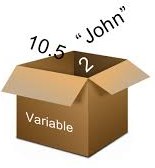
\includegraphics[trim=0 0 0 45,width=0.28\textwidth]{images/variables/variables}
\end{wrapfigure}
Le but d'un programme est de transformer de l'information. En général, un programme va commencer par stocker en mémoire les données d’entrée qui seront utilisées lors des étapes de traitement. Pour accéder à ces espaces de stockage et savoir quelle genre d'information ils contiennent, il va falloir leur attribuer un \textbf{nom} (ou \textbf{identifiant}) ainsi qu'un \textbf{type}. Pour finir, leur valeur va varier au fil de l'exécution du programme, c'est pourquoi on les appelle des \textbf{variables}. Chaque fois qu'on modifie la valeur d'une variable, on dit qu'on lui \textbf{affecte} une nouvelle valeur.
\begin{mydefinitions}
	\item  Une \textbf{variable} est un nom associé à un emplacement de la mémoire. C’est comme une boîte que l’on identifie par une étiquette. On dit aussi que le \textbf{nom de la variable est son identifiant}.
	\item Une \textbf{affectation} est l’attribution d’une valeur (d’un contenu) à une variable
\end{mydefinitions}
Pour résumer, une variable est décrite par
\begin{itemize}
	\item Un \textbf{identifiant} unique qui la désigne.
	\item Un \textbf{type} qui définit de quel « genre » est l’information associée.
	\item Une \textbf{valeur} qui doit respecter le type.
\end{itemize}


\vspace{1cm}
\act Indiquez le type des variables permettant de stocker (sur votre smartphone) les informations suivantes :
\begin{enumerate}
	\item le nom d’un contact
	\item l’heure du réveil
	\item un SMS
	\item le code de votre de votre compte eduge
	\item le pourcentage affiché de batterie restante
	\item la note de votre dernière évaluation de Mathématiques
	\item l'énoncé d'un devoir d'Histoire
	\item le fait que vous ayez déjà fini (ou non) ce devoir
\end{enumerate}

\vspace{1cm}

\newpage

\begin{wrapfigure}[]{r}{0.3\textwidth}
	\centering
	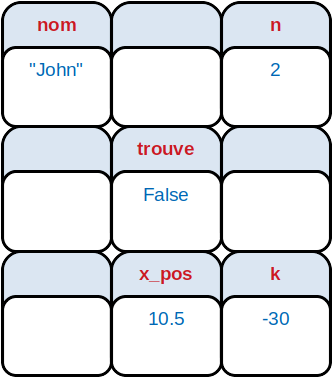
\includegraphics[width=0.28\textwidth]{images/variables/memoire}
	\caption{\small Représentation d'une mémoire d'ordinateur  comme des boîtes. Lorsqu'une variable est crée la boite obtient une \textit{étiquette} (en rouge) et une valeur (en bleu).}
\end{wrapfigure}
Il faut imaginer la mémoire de l’ordinateur comme une grosse armoire avec plein de petites boîtes. 
Certaines de ces boîtes ont un nom (une étiquette) : ce sont des variables, et elles peuvent contenir une valeur. Chaque fois que l'on a besoin de stocker une donnée on va créer une nouvelle variable, en programmation on dira que l'on \textbf{déclare} une variable.

En Python la déclaration d’une variable (et son typage) se fait dynamiquement à l’exécution du programme dès que cette variable apparaît dans une ligne de code. En fait, il suffit d'une \textbf{affectation} en utilisant le symbole "\lstinline{=}". Le code
\begin{lstlisting}[numbers=none]
myInt = 4
myString = "hello"
myReal = 2.5
\end{lstlisting}
crée 3 variables avec comme identifiant \lstinline{myInt}, \lstinline{myString} et \lstinline{myFloat} qui sont de type \lstinline{int}, \lstinline{str} et \lstinline{float} et qui contiennent les données \lstinline{4}, \lstinline{"hello"} et \lstinline{2.5}. 
\begin{center}
	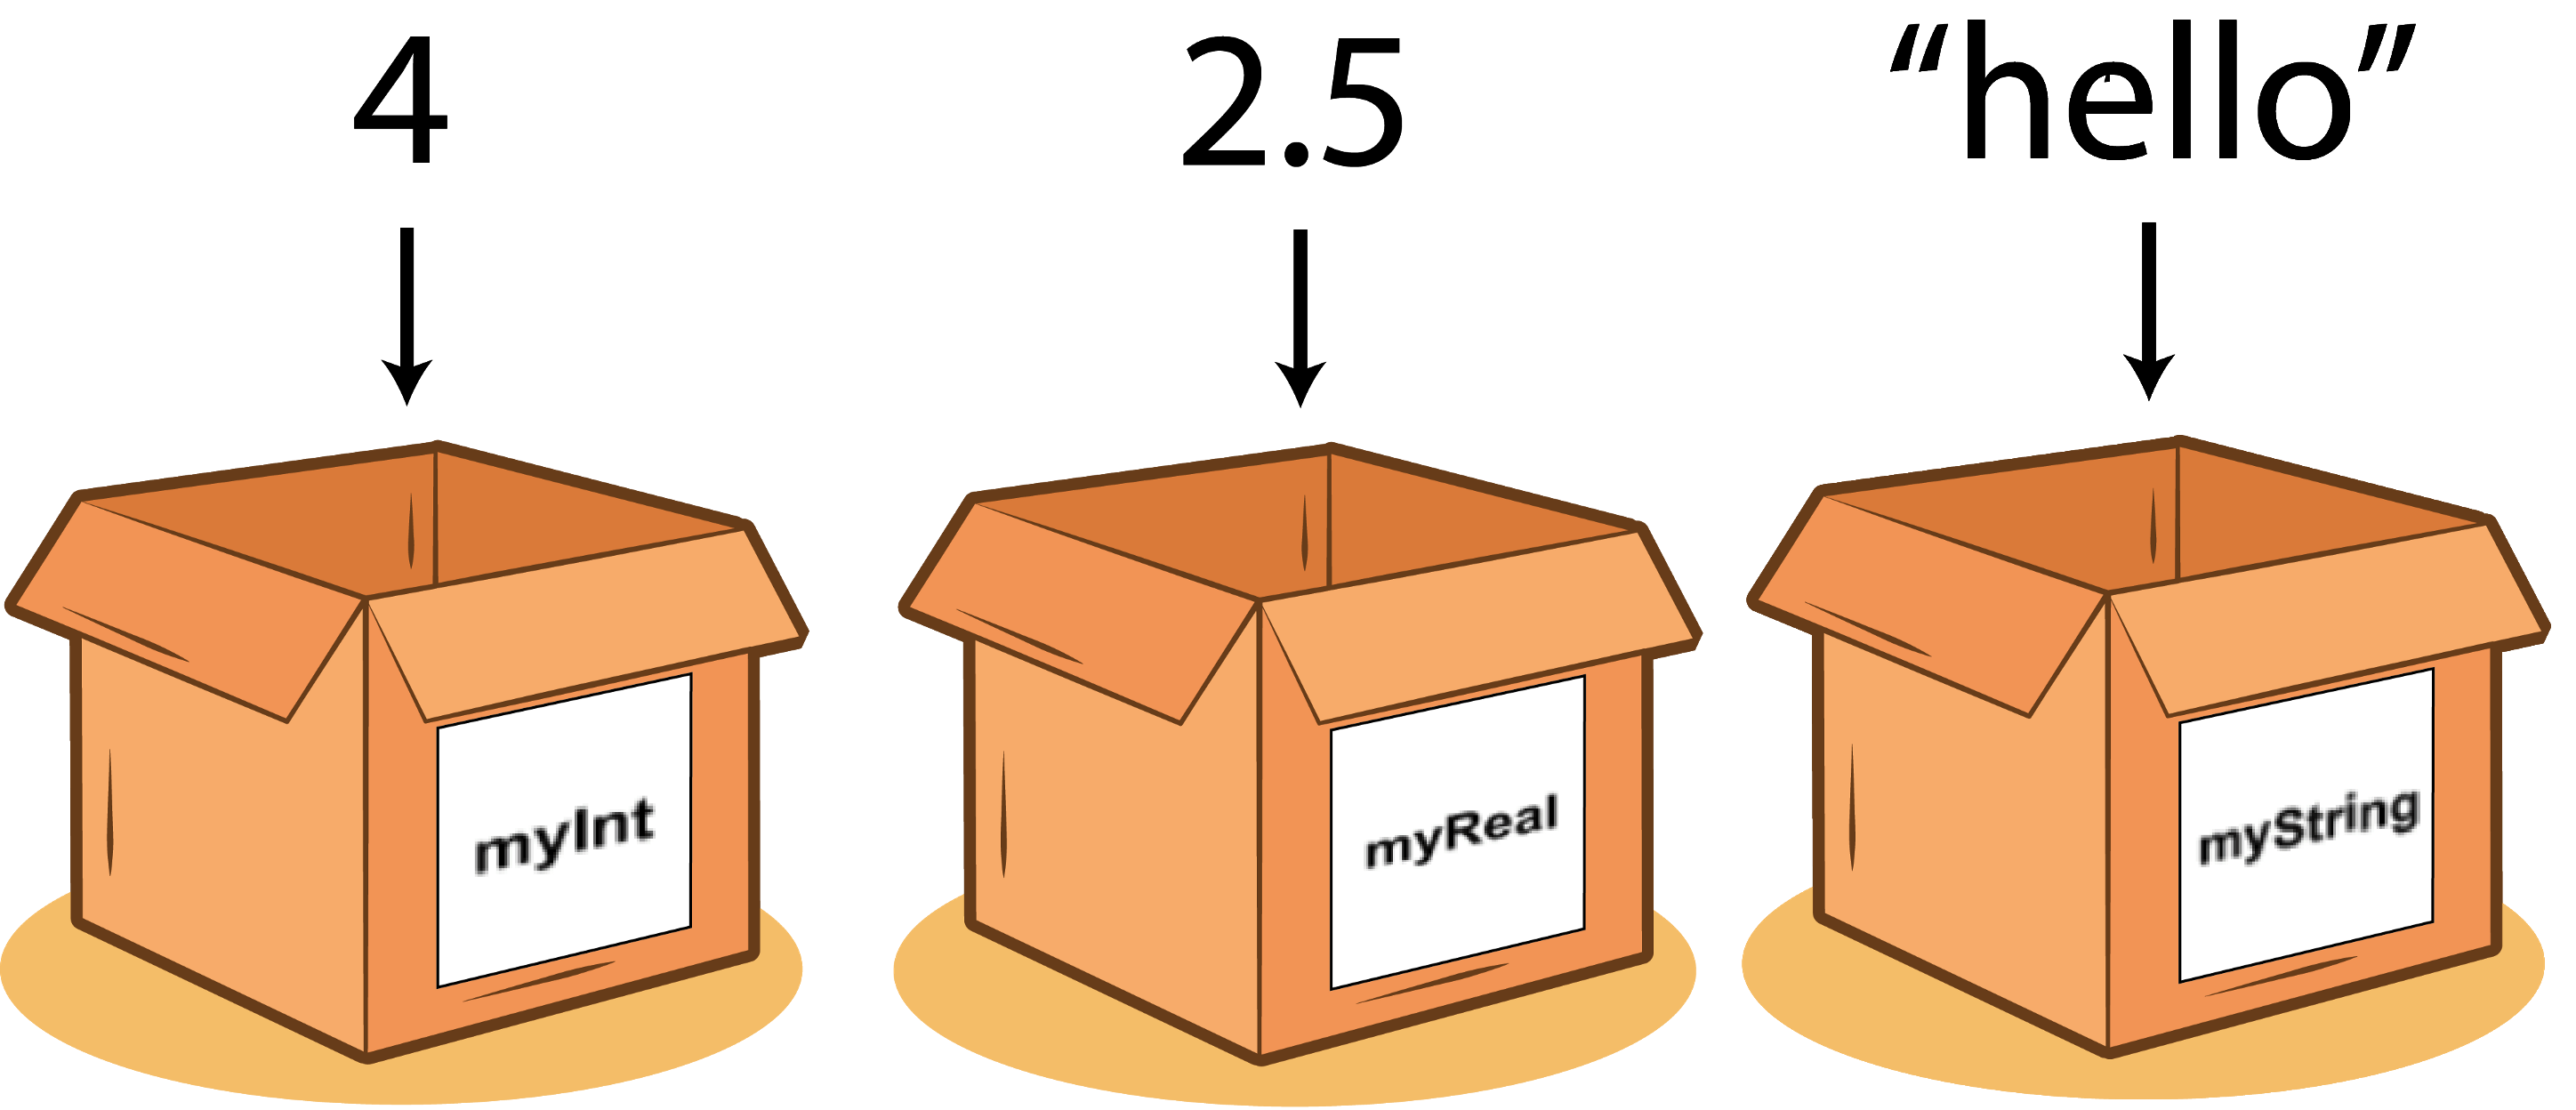
\includegraphics[trim=0 0 0 45,width=0.4\textwidth]{images/variables/variables2}
\end{center}

\begin{important}
	En Python, les noms de variables doivent en outre obéir à quelques règles simples :\\
	\begin{itemize}
		\item Il est exclusivement composé de lettres (majuscules  et/ou minuscules) et de chiffres mais doit toujours	commencer par une lettre.
		\item On ne peut pas utiliser l’un des 33 mots réservés du langage Python
		\begin{multicols}{7}
			\lstinline{and}\\      \lstinline{as}\\         \lstinline{assert}\\      \lstinline{break}\\       \lstinline{class}\\       \lstinline{continue}\\       \lstinline{def}\\
			\lstinline{del}\\       \lstinline{elif}\\       \lstinline{else}\\        \lstinline{except}\\      \lstinline{False}\\       \lstinline{finally}\\        \lstinline{for}\\
			\lstinline{from}\\      \lstinline{global}\\     \lstinline{if}\\          \lstinline{import}\\      \lstinline{in}\\          \lstinline{is}\\             \lstinline{lambda}\\
			\lstinline{None}\\      \lstinline{nonlocal}\\   \lstinline{not}\\         \lstinline{or}\\          \lstinline{pass}\\        \lstinline{raise}\\          \lstinline{return}\\
			\lstinline{True}\\      \lstinline{try}\\        \lstinline{while}\\     \lstinline{with}\\ \lstinline{yield}
		\end{multicols}	
		\item Le Seul symbole autorisé est le tiret du bas "$\_$" (underscore en anglais).
		Tous les autres caractères spéciaux sont interdits, en particulier l’espace blanc " " !
		\item Il est sensible à la casse : les minuscules sont différentes des MAJUSCULES. Exemple : les identifiant \lstinline{Age} et \lstinline{age} vont désigner des variables différentes.
	\end{itemize}
\end{important}

\begin{eclairage}
	Il est très important de donner un nom clair et précis aux variables. En lisant le nom de la variable, il faudrait avoir une idée de ce qu'elle représente.
	Par exemple, si je lis \lstinline{note_eleve_JohanS}, je me dis que cette variable représente la note de l'élève Johan S. et donc c'est probablement un \lstinline{float} entre 0.0 et 6.0. Pour améliorer la lecture, on utilise le seul symbole autorisé l'\textit{underscore} "$\_$"\\
\end{eclairage}


\subsection{L'affectation}
Chaque variable (déclarée) possède une valeur qui est l’information qu’elle porte. Par exemple, la valeur de la variable \lstinline{nombre_eleves_GR103} pourrait être 23, celle de la variable \lstinline{note} pourrait être 4.5, celle de la variable \lstinline{prenom} pourrait être "Anouk".
En Python, pour définir ou modifier la valeur d’une variable, il suffit de lui affecter une valeur en utilisant le symbole égal "\lstinline{=}". 
\begin{mydefinition}
	L’\textbf{affectation} d’une valeur à une variable est l’instruction basique qui permet d’attribuer une valeur à une variable. Par abus de langage, on dit souvent «affectation de variable» ou «assignation de variable».
\end{mydefinition}
En Python, l'affectation s’effectue avec l’opérateur \lstinline{=}. L'instruction d'affectation est composée d'une variable, suivie du symbole  \lstinline{=} et d'une expression à évaluer. Après avoir exécutée une affectation la variable prendra la valeur de l'expression évaluée.
\begin{myexample}
	\begin{lstlisting}[numbers=none]
>>> x = (1 + 2) * (3 + 4)
>>> print(x)
21
	\end{lstlisting}
\end{myexample}

\begin{important}
	\begin{itemize}
		\item 	Il ne faut pas confondre l'opérateur \lstinline{=} (l'affectation) et l'opérateur \lstinline{==} qui sert à tester l'égalité de deux valeurs. L'opérateur \lstinline{==} est beaucoup plus proche du concept d'égalité utilisée en mathématiques.
		\item Il est important de distinguer les expressions, comme \lstinline{x + 2} , des instructions, comme \lstinline{y = x + 2}; . Une expression se calcule, une instruction s’exécute.
	\end{itemize}
	
\end{important}

\subsection{Différents types d’affectations}

\begin{myexamples}
	\itemb{Affectation d'une quantité}
	\begin{lstlisting}[numbers=none]
note = 37 * 50 + 1
	\end{lstlisting}
	\textbf{Explications :}
	\begin{minipage}[t]{0.83\linewidth}
		La valeur \lstinline{37* 50 + 1} (c'est-à-dire \lstinline{4.7}) est injectée dans la case mémoire nommée \lstinline{note}.
	\end{minipage}	
	
	\itemb{Affectation d’un texte}
	\begin{lstlisting}[numbers=none]
prenom = "Robert"
nom_prenom = "Dupont"+'Robert'
	\end{lstlisting}
	\textbf{Remarque :}
	\begin{minipage}[t]{0.85\linewidth}
		Un Chaîne de caractères peut être écrite soit entre "guillemets", soit entre 'apostrophes' droits.
	\end{minipage}
	
	
	\itemb{Affectations parallèles}
	\begin{lstlisting}[numbers=none]
n, x = 1, 7.3
	\end{lstlisting}
	\textbf{Explications :}
	\begin{minipage}[t]{0.83\linewidth}
		C'est équivalent à effectuer les affectations \lstinline{n = 1} et  \lstinline{x = 7.3} simultanément.
	\end{minipage}	
	
	
	\itemb{Auto-affectation}
	\begin{lstlisting}[numbers=none]
k = k ** 2
t = 3 * t - 2
	\end{lstlisting}
	\textbf{Explications :}
	\begin{minipage}[t]{0.83\linewidth}
		Une expression avec la valeur de la variable est calculée puis réaffectée à la variable elle-même.\\
		Par exemple, si \lstinline{t} contient la valeur $5$ alors après avoir exécute \lstinline{t=3*t-2} \lstinline{t} vaudra  \lstinline{3*5-2} (c'est-à-dire \lstinline{13}). 
	\end{minipage}
	
	
	
	\itemb{Incrémentation ou décrémentation}
	\begin{lstlisting}[numbers=none]
k = k + 1
compteur = compteur - 2
	\end{lstlisting}
	\textbf{Remarque :}
	\begin{minipage}[t]{0.85\linewidth}
		Auto-affectation additionnée ou soustraite d’un certain \textit{pas} (d’un certain nombre) entier.
	\end{minipage}
\end{myexamples}


\end{document}